\section{Eigenschaften}
\subsection{Gleichungen {\formelbuch{248, Mittelwerte: 19ff}}}
\begin{tabular}{llll}
  \textbf{Tangentengleichung} &
  \textbf{Normalengleichung} &
  \textbf{Linearer Mittelwert} &
  \textbf{Quadratischer Mittelwert}\\
  $y-y_0=f'(x_0)(x-x_0)$ &
  $y-y_0=-\frac{1}{f'(x_0)}(x-x_0)$ &
  $\bar{f} = \frac{1}{b-a} \int\limits_{a}^{b} f(x)dx$ &
  $\bar{f} = \sqrt{\frac{1}{b-a} \int\limits_{a}^{b} f(x)^2dx}$
\end{tabular}
  
\subsection{Tangenten- \& Normalenabschnitt, Subtangente \&
Subnormale \formelbuch{249ff}}

\subsection{Abstandsformeln}
\begin{minipage}{6.5cm}
    \textbf{Hessesche Normalform \formelbuch{200f, 222}}\\
    $x\cdot \cos\varphi_0 +y\cdot \sin\varphi_0=r_0$\\
    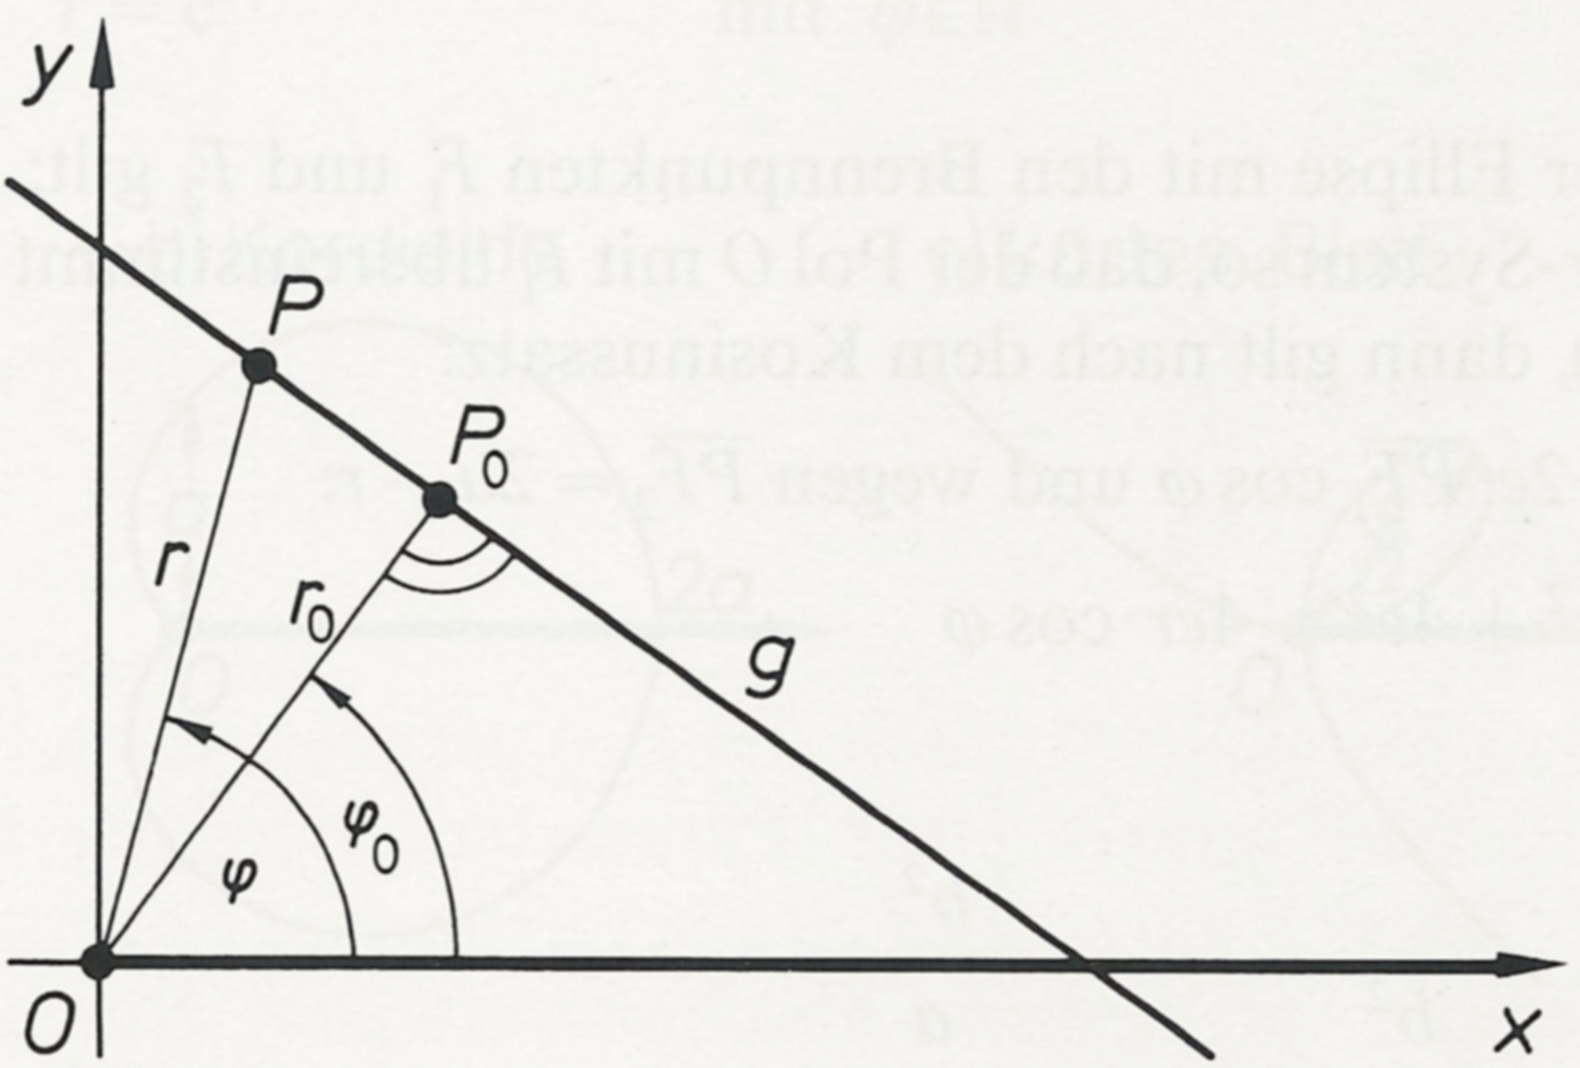
\includegraphics[width=2.8cm]{./bilder/hessenorm.png}
\end{minipage}
\begin{minipage}{6.5cm}
  \textbf{Geradengleichung} \\
  $y - y_0 = m (x - x_0)$
\end{minipage}
\begin{minipage}{6cm}
  \textbf{Abstand zum Ursprung} \\
  $\frac{|y_0 - m \cdot x_0|}{\sqrt{m^2 + 1}}$
\end{minipage}

\subsection{Ber"uhrung h"oherer Ordnung}
Zwei explizit gegebene Kurven $y = f(x)$ und $y = g(x)$ ber"uhren einander im
Punkt P $x_0, y_0$ von der Ordnung $n$, wenn die Funktionswerte und die ersten
$n$ Ableitungen existieren und übereinstimmen.\\
$f(x_0) = g(x_0);\; f'(x_0) = g'(x_0);\; f''(x_0) = g''(x_0);\;\ldots ;
\;f^{(n)}(x_0) = g^{(n)}(x_0)\; \qquad f^{(n+1)}(x_0) \neq g^{(n+1)}(x_0)$

\subsection{Scheitel \formelbuch{254}}
Scheitelpunkte sind Extremalwerte der Kr"ummungs- bzw. Kr"ummungsradiusfunktion.
Falls bei $\kappa'(x)$ an der Stelle $x_0$ ein Vorzeichenwechsel besteht, existiert dort
eine Extremalstelle. 

\subsection{Kr"ummung \formelbuch{????}}
\begin{tabular}{l|c|r}
  $\kappa > 0 \quad\Rightarrow$ \quad Linkskr"ummung $\iff$ konvex &
  $\kappa = 0 \quad\Rightarrow$ \quad Wendepunkt \quad & \quad
  $\kappa < 0 \quad\Rightarrow$ \quad Rechtskr"ummung $\iff$ konkav
  \\ 
\end{tabular}

%\subsection{Wichtige Formeln\formelbuch{FF S60}}
%Siehe Tabelle \ref{wichtige_formeln} im Ahnang.

\subsection{Orthogonale Trajektorien \formelbuch{????}}
	\begin{minipage}{.2\textwidth}
		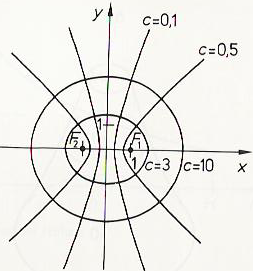
\includegraphics[height=3.5cm]{bilder/orthoTrajekt_klein.png}
	\end{minipage}%
	\begin{minipage}{.8\textwidth}
		Die orthogonalen Trajektorien schneiden alle Kurven der gegebenen Kurvenschar
		$y=f(x,c)$ im rechten Winkel.\\
		\textbf{Vorgehen:} \\
		1. c eliminieren: $y$ ableiten, nach c auflösen und in $y$ einsetzten
		$\Rightarrow$ DGL: $F(x,y,y')$ \\
		2. $y'$ durch $-\frac{1}{'y}$ ersetzen. \\
		2. DGL auflösen (sofern nötig...)\\
	\end{minipage}

